% =========================================================================== %

\begin{frame}[t,plain]
\titlepage
\end{frame}

% =========================================================================== %

\begin{frame}{Recap}
%
\begin{columns}[T]
\column{.5\linewidth}
\texttt{pd.Series}
\begin{itemize}
\item Represents One Column of Data
\item Built on NumPy Arrays
\item Arbitrary Indices
\item Element-Wise Operations
\item Index Alignment
\item Reduction Functions
\item Boolean Array Indexing
\end{itemize}
%
\column{.5\linewidth}
\texttt{pd.DataFrame}
\begin{itemize}
\item Represents a Table of Data
\item Collection of \texttt{pd.Series}
\item Reader and Writer for Many Standard Formats
\item Non-Owning Views
\item Grouping, Binning and Sorting
\item Iterating over Data
\item Connection to MatPlotLib
\end{itemize}

\end{columns}
%
\begin{center}
	\emph{Any Questions?}
\end{center}
%
\end{frame}

% =========================================================================== %

\begin{frame}{Old Files}
%
\begin{columns}[T]
\column{.22\linewidth}
\includegraphics[width=\linewidth]{./gfx/xkcd-oldfiles}
%
\column{.5\linewidth}
\begin{center}
\emph{Wow, ANIMORPHS-NOVEL.RTF? Just gonna, uh, go through and delete that from all my archives real quick.}

\vspace{12pt}
Source: \url{https://xkcd.com/1360/}
\end{center}
\end{columns}
%
\end{frame}

% =========================================================================== %

\begin{frame}
%
\begin{center}
	\includegraphics[width=.9\linewidth, page=1]{./gfx/filesystems}
\end{center}
%
\end{frame}

% =========================================================================== %

\begin{frame}{Structure Elements of a Partition}
%
\begin{columns}
\column{.7\linewidth}
	\includegraphics[width=\linewidth, page=2]{./gfx/filesystems}
%
\column{.3\linewidth}
	\small
	\begin{itemize}
	\item There can be multiple file systems (partitions) on a single physical device.
	\item There are dozens of file systems, all with their particular inner workings
	\item The scheme holds for most common file systems, such as NTFS, ext3 or ext4
	\item We could do an entire lecture \emph{series} on file systems alone
	\end{itemize}
\end{columns}
%
\end{frame}

% =========================================================================== %

\begin{frame}{Regular Files and Fragmentation}
%
% trim = left bottom right top
\includegraphics[width=\linewidth, page=3,trim=0 300 0 20,clip]{./gfx/filesystems}
%
\begin{columns}
\column{.5\linewidth}
	\begin{itemize}
	\item List of entries: tuples of strings and inodes
	\item Inodes: Metadata and actual location: block ID
	\end{itemize}
%
\column{.5\linewidth}
	\begin{itemize}
	\item Blocks: fixed size
	\item Larger files: multiple blocks
	\item[\Thus] Fragmentation
	\end{itemize}
\end{columns}
%
\end{frame}

% =========================================================================== %

\begin{frame}{Hardlinks}
%
% trim = left bottom right top
\includegraphics[width=\linewidth, page=4,trim=0 300 0 20,clip]{./gfx/filesystems}
%
\begin{columns}
\column{.5\linewidth}
	\begin{itemize}
	\item Multiple entries in List of Entries can point to same inode
	\item[\Thus] Same file in two (or more) locations
	\item Changes affect both locations
	\end{itemize}
%
\column{.5\linewidth}
	\begin{itemize}
	\item Imagine shared ressource for several project folders
	\item File is only deleted when all references are removed
	\end{itemize}
\end{columns}
%
\end{frame}

% =========================================================================== %

\begin{frame}{Symbolic Links (aka SymLinks)}
%
% trim = left bottom right top
\includegraphics[width=\linewidth, page=5,trim=0 300 0 20,clip]{./gfx/filesystems}
%
\begin{columns}
\column{.5\linewidth}
	\begin{itemize}
	\item Speical kind of inode
	\item Content: referenced file
	\item In principle same effect
	\end{itemize}
%
\column{.5\linewidth}
	\begin{itemize}
	\item Moving/Deleting original file breaks the link
	\item Works across file systems
	\end{itemize}
\end{columns}
%
\end{frame}

% =========================================================================== %

\begin{frame}{Link Files}
%
% trim = left bottom right top
\includegraphics[width=\linewidth, page=6,trim=0 300 0 20,clip]{./gfx/filesystems}
%
\begin{columns}
\column{.5\linewidth}
	\begin{itemize}
	\item Like SymLinks, but done in regular files
	\item Treated by GUI rather than OS
	\item Same (dis)advantages
	\end{itemize}
%
\column{.5\linewidth}
	\begin{itemize}
	\item Windows: \texttt{.lnk} files
	\item Linux: \texttt{.desktop} files
	\item Mac: I don't have a fucking clue
	\end{itemize}
\end{columns}
%
\end{frame}

% =========================================================================== %

\begin{frame}
%
\begin{columns}
\column{.5\linewidth}
\begin{hintbox}[Following Symlinks and Link Files]
	Not all programs automatically follow symlinks. \emph{Most} programs don't follow link files. One example is a zip program I was using two years ago, to the effect
	that I nearly failed a course.\\
	
	You can find out about the nature by visual clues: in Windows, link files and symlinks are rendered with an arrow in the lower left corner.
	Depending on your file browser, symlinks sometimes are rendered in different colours.\\
	
	In the console, \texttt{ls -l} (Linux/Mac) or \texttt{dir /a} (Windows) reveals the true nature of a file.
\end{hintbox}
%
\column{.5\linewidth}
	\begin{center}
		
\includegraphics[width=.4\linewidth]{./gfx/link-folder}
	\end{center}
	
	\begin{center}
		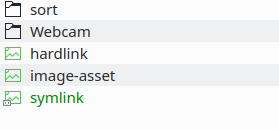
\includegraphics[width=.8\linewidth]{./gfx/link-linux}
	\end{center}
	
	\begin{center}
		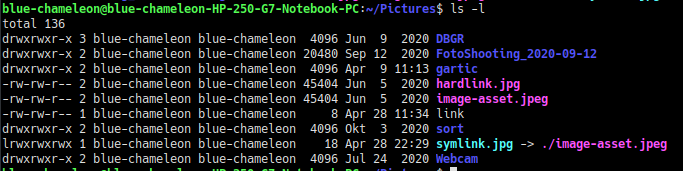
\includegraphics[width=1.\linewidth]{./gfx/link-konsole}
	\end{center}
	
	
\end{columns}
%
\end{frame}

% =========================================================================== %

\begin{frame}{Todays Modules}
%
\begin{itemize}
\item \texttt{os} -- Operating System Functions
	\begin{itemize}
	\item Common interface to OS-specific calls
	\item Mostly: deal with the file system
	\item \url{https://docs.python.org/3/library/os.html}
	\item Submodule \texttt{path}
	\item \url{https://docs.python.org/3/library/os.path.html}
	\end{itemize}
\item \texttt{glob} -- Frontend for \texttt{os}
	\begin{itemize}
	\item Easy traversal of folder structures
	\item \url{https://docs.python.org/3/library/glob.html}
	\end{itemize}
\item \texttt{sys} -- Python Interna
	\begin{itemize}
	\item Command line parameters
	\item Memory model
	\item Default behaviour
	\item \url{https://docs.python.org/3/library/sys.html}
	\end{itemize}
\end{itemize}
%
\end{frame}

% =========================================================================== %

\begin{frame}{Controlling Directories}
%
\begin{itemize}
\item \texttt{os.chdir(path)} -- change CWD to \texttt{path}, given as string
\item \texttt{os.getcwd()} -- find out CWD as string
\item \texttt{os.curdir} and \texttt{os.pardir} -- string constants \inPy{'.'} and \inPy{'..'}
\item \texttt{os.mkdir(subfolder)} -- create \texttt{subfolder} under the CWD, where subfolder is a string
\item \inPy{os.makedirs("multiple/subdirs/at/once")}
\item \texttt{os.rmdir(directory)} -- delete \emph{empty} directory, given as string
	\begin{itemize}
	\item May neither contain files nor subdirectories
	\item Otherwise raises \texttt{OSError: [Errno 39] Directory not empty: 'directory'}
	\end{itemize}
\end{itemize}
%
\end{frame}

% =========================================================================== %

\begin{frame}{Controlling Files}
%
\begin{itemize}
\item \texttt{os.remove(filename)} -- delete a file
\item \texttt{os.rename(src, dst)} -- change filename or move a file
	\begin{itemize}
	\item E.\;g.: \inPy{os.rename("./sourceDir/file", "./destinationDir/newName")}
	\end{itemize}
\item \texttt{os.link(source, link)} -- creates a hardlink from \texttt{sorce} with name \texttt{link}, both strings
\item \texttt{os.symlink(source, link)} -- creates a hardlink from \texttt{sorce} with name \texttt{link}, both strings
\item Remember: Create files with Python's \inPy{open} command
\end{itemize}
%
\end{frame}

% =========================================================================== %

\begin{frame}[fragile]{Traversing the File System}
%
\begin{itemize}
\item \inPy{os.listdir(path='.')}
	\begin{itemize}
	\item Returns a \inPy{list} of strings
	\item All elements in the CWD
	\item Regardless of type (file, symlink, directory)
	\item Does not contain \inPy{'.'} and \inPy{'..'}
	\end{itemize}
\item \inPy{os.scandir(path='.')}
	\begin{itemize}
	\item Returns iterator to \texttt{os.Direntry} object
	\item Object has \inPy{__enter__} and \inPy{__exit__}, \ie is compatible with \inPy{with}:\\
\begin{minted}{python3}
with os.scandir() as it :
    for entry in it :
        ...
\end{minted}
	\end{itemize}
\item For both of them
	\begin{itemize}
	\item No particular order
	\item Neither of them supports wildcards (\texttt{*} or \texttt{?})
	\end{itemize}
\end{itemize}
%
\end{frame}

% =========================================================================== %

\begin{frame}{Traversing the File System: The \texttt{Direntry} Object}
%
\inPy{it = os.scandir()}
\begin{itemize}
\item Iterator -- \inPy{for entry in it:} or \inPy{entry = next(it)}
\item \inPy{entry.name} -- file name as string, relative to path in \texttt{scandir}
\item \inPy{entry.path} -- full file name, including path, as string
\item \inPy{entry.is_dir()}, \inPy{entry.file()}, \inPy{entry.symlink()} -- booleans, identifying the kind of entry
\item \inPy{entry.file(follow_symlinks=True)}
	\begin{itemize}
	\item If \inPy{follow_symlinks=True}: returns \inPy{True} only if symlink is not broken
	\item Otherwise: Returns \inPy{False} when encountering a symlink
	\end{itemize}
\item \texttt{it.close()}
	\begin{itemize}
	\item Ends iteration, frees ressources
	\item Not needed when used in \inPy{with} block
	\item \enquote{Only} slows down OS when forgotten
	\end{itemize}
\end{itemize}
%
\end{frame}

% =========================================================================== %

\begin{frame}{Traversing the File System: \texttt{glob} Module}
%
\begin{itemize}
\item Often: Need to filter for a certain file type (\eg \texttt{.jpg} files)
\item Or: Need to traverse \emph{recursively} (subfolders of subfolders of ...)
\item[\Thus] Module \texttt{glob} provides solutions, built from \texttt{os}
\item \inPy{glob.glob(path, recursive=False)}
	\begin{itemize}
	\item Return a (possibly empty) \inPy{list} of strings
	\item Relative to \texttt{path}
	\item May contain Wildcards
	\item If \inPy{recursive=True}, subfolders are explored, too
	\item Broken symlinks are included
	\end{itemize}
\end{itemize}
%
\end{frame}

% =========================================================================== %

\begin{frame}{Wildcards}
%
\begin{itemize}
\item Like escape characters -- stand in characters
\item \texttt{?} -- an arbitrary character
	\begin{itemize}
	\item E.\;g. \texttt{myFile-?.ext} matches \texttt{myFile-a.ext}, \texttt{myFile-A.ext}, \texttt{myFile-0.ext}, ... but not \texttt{myFile-aa.ext} or
	\texttt{myFile-.ext}
	\end{itemize}
\item \texttt{*} -- any number of arbitrary characters
	\begin{itemize}
	\item E.\;g. \texttt{*.jpg} matches \emph{all} \texttt{jpg} files
	\item E.\;g. \texttt{a*.ext} matches \texttt{abcde.ext} and even \texttt{a.ext}
	\end{itemize}
\item \texttt{**} -- any number of subdirectories (including zero)
	\begin{itemize}
	\item Only when \inPy{recursive = Tuue}
	\end{itemize}
\item \texttt{[wildcard]} -- literal matching
\end{itemize}
%
\begin{hintbox}[Rules for Filenames]
If your filenames contain ?, *, <, |, >, [, ], /, \, " or \$, you're using your computer wrong.
\end{hintbox}
%
\end{frame}

% =========================================================================== %

\begin{frame}[fragile]
%
\begin{tcbraster}[raster columns=2,
                  raster equal height,
                  nobeforeafter,
                  raster column skip=0.5cm]
\begin{codebox}[Beispiel: Title goes here]
\begin{minted}[fontsize=\scriptsize, linenos]{python3}
foo
\end{minted}
\end{codebox}
%
\begin{codebox}[Beispiel: Title goes here]
\begin{minted}[fontsize=\scriptsize, linenos]{python3}
bar
\end{minted}
\end{codebox}
\end{tcbraster}
%
\end{frame}

% =========================================================================== %

\begin{frame}[fragile]{Kapitel 6}
%
\begin{itemize}
\item Optionale Parameter
\item Variadische Funktionen
\item Funktionen als Rückgabewerte
\item Lambdas
\item Rekursion
\end{itemize}
%
\end{frame}

% =========================================================================== %

\begin{frame}[fragile]{\inPy{while}-Schleifen}
%
\begin{columns}[T]
\column{.5\linewidth}
\begin{itemize}
\item x
\end{itemize}
%
\column{.5\linewidth}
\begin{codebox}[Syntax: Title goes here]
\begin{minted}[fontsize=\scriptsize]{python3}
Stuff
\end{minted}
\end{codebox}
\end{columns}
%
\end{frame}

% =========================================================================== %

\begin{frame}[fragile]
%
\begin{codebox}[Beispiel: Title goes here]
\begin{minted}[linenos, fontsize=\scriptsize]{python3}
x
\end{minted}
\end{codebox}
%
\end{frame}
